
% This LaTeX was auto-generated from an M-file by MATLAB.
% To make changes, update the M-file and republish this document.

\documentclass{article}
\usepackage{graphicx}
\usepackage{color}

\sloppy
\definecolor{lightgray}{gray}{0.5}
\setlength{\parindent}{0pt}

\begin{document}

    
    

\section*{Plot graph}

\begin{par}
Creates plot
\end{par} \vspace{1em}
\begin{verbatim}
clear all;
close all;

snr_dB = -5:5:30;
%snr_dB = snr_dB + 5;

[filename, pathname] = uigetfile('*.mat', 'Select data files', 'Multiselect', 'on')
files = strcat(char(pathname), filename);
b = [];
x = [];
s = [];
for i = 1:size(files, 2)
    load(files{i},'ber*', 'pt_bits');
    b = [b,ber_pu_direct];
    x = [x,ber_pu_relay];
    s = [s,ber_su];

end
ber_pu_direct = b;
ber_pu_relay = x;
ber_su = s;

throughput_pu_direct = 6*(1-ber_pu_direct);
throughput_pu_relay = 6*(1-ber_pu_relay);
throughput_su = 6*(1-ber_su);

figure
semilogy(snr_dB, ber_pu_direct, 'r')
hold on
semilogy(snr_dB, ber_pu_relay, 'g')
hold on
semilogy(snr_dB, ber_su)
legend('BPSK Primary System', 'Relayed Primary System', 'Secondary System');
grid on;

figure
plot(snr_dB, throughput_pu_direct, 'r')
hold on
plot(snr_dB, throughput_pu_relay, 'g')
hold on
plot(snr_dB, throughput_su)
axis([snr_dB(1) snr_dB(end) min([throughput_pu_direct throughput_pu_relay throughput_su])-0.5 max([throughput_pu_direct throughput_pu_relay throughput_su])+0.5])
legend('BPSK Primary System', 'Relayed Primary System', 'Secondary System');
grid on;
\end{verbatim}

        \color{lightgray} \begin{verbatim}
filename = 

    [1x45 char]    [1x45 char]    [1x45 char]


pathname =

C:\Users\Prabhpreet\OneDrive\College\Research\Project\MATLAB\Basic_Relay_with_STBC\cooperativespectrumsharing\value_archive\050115\

\end{verbatim} \color{black}
    
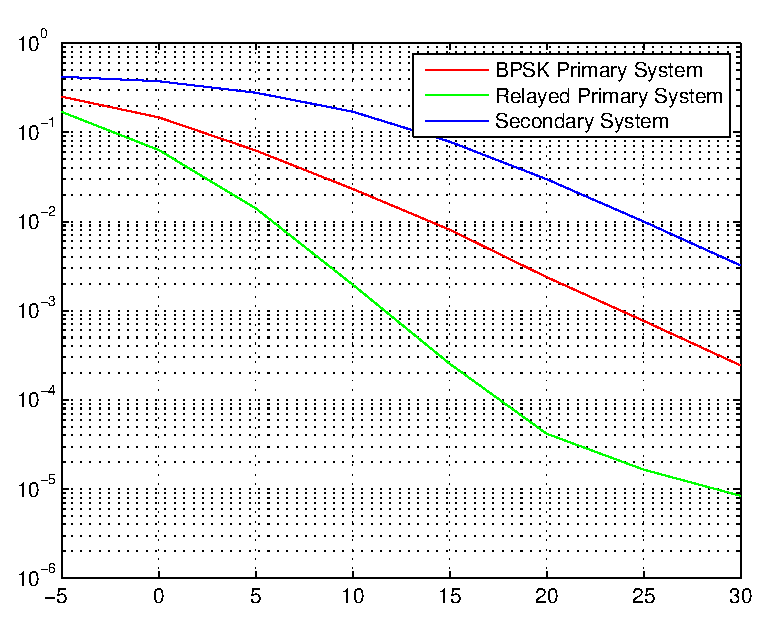
\includegraphics [width=4in]{plot_graph_01.eps}

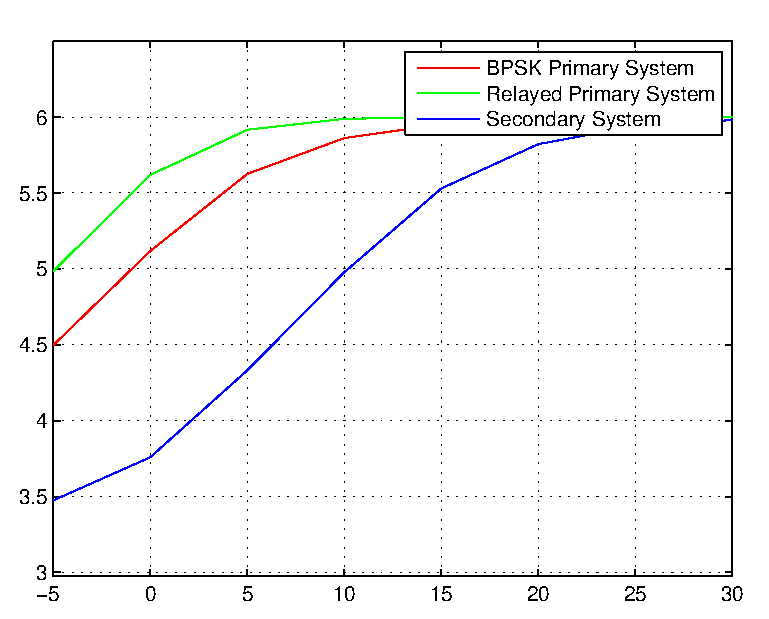
\includegraphics [width=4in]{plot_graph_02.eps}



\end{document}
    
